\documentclass[aspectratio=169,11pt]{beamer}
\usepackage[utf8]{inputenc}
\usepackage[T1]{fontenc}
\usepackage[brazil]{babel}
\usepackage{booktabs}
\usepackage{array}
\newcolumntype{L}[1]{>{\raggedright\arraybackslash}p{#1}}
\usepackage{graphicx}
\usepackage{tikz}
\usetikzlibrary{arrows.meta,positioning,fit,calc}

\usetheme{default}
\usecolortheme{default}
\setbeamertemplate{navigation symbols}{}
\setbeamertemplate{footline}[frame number]
\definecolor{azul}{RGB}{31,78,121}
\definecolor{verde}{RGB}{46,125,50}
\definecolor{cinza}{RGB}{235,235,235}
\setbeamercolor{frametitle}{fg=azul}
\setbeamercolor{title}{fg=azul}
\setbeamerfont{frametitle}{series=\bfseries}
\newcommand{\code}[1]{\texttt{\detokenize{#1}}}

\title{Verificação UVM do sistema RISC-V + DMA + malha sistólica}
\subtitle{Trabalho final de Verificação --- ambiente do top-level}
\author{Equipe: \textit{(preencher)}}
\date{Dezembro de 2026}

\begin{document}

\begin{frame}
\titlepage
\end{frame}

% ---------------------------------------------------------------- 2
\begin{frame}{O que está sendo verificado}
\begin{columns}[T]
\begin{column}{0.48\textwidth}
\small
O sistema calcula $C = A \times B$:
\begin{itemize}
  \item a \textbf{CPU} RV32I roda o firmware: escreve nos registradores do DMA os endereços e as
  dimensões e dá START;
  \item o \textbf{DMA} move tudo sozinho: lê $A$ e $B$, alimenta a malha, soma as parciais e
  escreve $C$;
  \item a \textbf{malha sistólica} tem $S \times S$ elementos ($S$ = 2, 4 ou 8); matrizes maiores
  são divididas em blocos.
\end{itemize}
O DUT é o \code{soc_top}: por fora só tem clock, reset e \code{irq_o}.
\end{column}
\begin{column}{0.5\textwidth}
\centering
\begin{tikzpicture}[font=\scriptsize,
  b/.style={draw,rounded corners=2pt,fill=white,align=center,minimum height=0.8cm},
  a/.style={-{Latex[length=1.6mm]},thick}]
\node[b,text width=1.6cm] (cpu) at (0,2.6) {CPU RV32I};
\node[b,text width=1.6cm] (im) at (2.6,2.6) {Memória de instruções};
\node[draw,fill=cinza,minimum width=6.0cm,minimum height=0.5cm] (bus) at (1.6,1.5)
  {Interconexão AXI4-Lite};
\node[b,text width=1.3cm] (dm) at (-0.6,0.2) {Memória de dados};
\node[b,text width=1.1cm] (dma) at (1.0,0.2) {DMA};
\node[b,text width=1.7cm] (acc) at (3.2,0.2) {Adaptador e malha $S{\times}S$};
\draw[a] (cpu) -- (im);
\draw[a] (cpu) -- (cpu |- bus.north);
\draw[a] (dm |- bus.south) -- (dm);
\draw[a,<->] (dma |- bus.south) -- (dma);
\draw[a] (acc |- bus.south) -- (acc);
\draw[a,dashed] (dma.south) -- ++(0,-0.4) -| node[pos=0.25,below]{\code{irq}} ($(cpu.west)+(-0.5,0)$) -- (cpu.west);
\end{tikzpicture}
\end{column}
\end{columns}
\end{frame}

% ---------------------------------------------------------------- 3
\begin{frame}{Como o estímulo entra}
\small
\begin{itemize}
  \item O DUT não tem portas de dados: o ambiente escreve $A$, $B$ e a descrição da operação
  \textbf{direto na memória} (backdoor) e lê $C$ do mesmo jeito.
  \item \textbf{Quem programa o DMA é sempre o firmware, pela CPU.} O ambiente não toca em
  registrador e não usa \code{force}.
  \item O firmware é \textbf{genérico}: lê um bloco de parâmetros no início da memória de dados.
\end{itemize}
\vspace{2mm}
\centering\footnotesize
\begin{tabular}{@{}lll@{}}
\toprule
Palavra & Campo & Quem escreve\\
\midrule
0 & \code{CMD} (1 = há operação) & ambiente; o firmware zera\\
1--6 & endereços de $A$, $B$, $C$; $M$, $K$, $N$ & ambiente\\
7 & \code{FLAGS}: interrupção; falhas injetadas & ambiente\\
8 & \code{STATUS} do DMA no fim & firmware\\
9 & \code{DONE_COUNT} & firmware, \textbf{depois} de zerar \code{CMD}\\
\bottomrule
\end{tabular}
\vspace{2mm}

\small Uma simulação roda quantas operações quiser, sem remontar o firmware.
\end{frame}

% ---------------------------------------------------------------- 4
\begin{frame}{Arquitetura do ambiente}
\centering
\begin{tikzpicture}[font=\scriptsize,
  c/.style={draw,rounded corners=2pt,fill=white,align=center,minimum height=0.7cm,inner sep=2pt},
  a/.style={-{Latex[length=1.5mm]},thick}]
\node[c,text width=1.6cm] (seq) at (0,3.2) {sequences\\(11)};
\node[c,text width=1.6cm] (sqr) at (0,2.0) {sequencer};
\node[c,text width=2.1cm,fill=blue!6] (drv) at (0,0.7) {driver\\\code{fw} ou \code{bfm}\\(factory)};
\node[c,text width=1.6cm] (mon) at (3.0,0.7) {monitor\\passivo};
\node[draw,dashed,fit=(sqr)(drv)(mon),inner sep=6pt,label={[font=\scriptsize,align=center]left:agente\\
  \code{mm_agent}}] {};
\node[c,text width=1.8cm,fill=green!8] (ref) at (6.0,2.4) {modelo de\\referência (TLM)};
\node[c,text width=1.6cm] (sb) at (8.6,1.4) {scoreboard};
\node[c,text width=1.6cm] (cov) at (6.0,0.2) {cobertura};
\node[c,text width=1.8cm] (aut) at (8.6,-0.4) {autonomia};
\node[c,text width=1.7cm] (bus) at (6.6,-1.5) {2 agentes AXI passivos};
\node[c,text width=6.2cm,fill=gray!15,minimum height=0.8cm] (dut) at (1.5,-1.5) {DUT
  \code{soc_top} (ou \code{soc_subsys} sem CPU)\\+ asserções de sistema por \code{bind}};
\draw[a] (seq) -- (sqr);
\draw[a] (sqr) -- (drv);
\draw[a] (drv) -- node[left,font=\tiny]{memória} (drv |- dut.north);
\draw[a] (mon |- dut.north) -- node[right,font=\tiny]{memória} (mon);
\draw[a] (mon) -- (ref);
\draw[a] (ref) -- node[above,font=\tiny]{esperado} (sb);
\draw[a] (mon) -- node[below,font=\tiny,pos=0.6]{observado} (sb);
\draw[a] (mon) -- (cov);
\draw[a] (bus) -- (aut);
\draw[a] (dut.east) -- (bus.west);
\end{tikzpicture}

\vspace{1mm}
\small Camadas em pacotes: \code{mm_agent_pkg} $\rightarrow$ \code{mm_env_pkg} $\rightarrow$
\code{mm_test_pkg}; teste por \code{+UVM_TESTNAME}.
\end{frame}

% ---------------------------------------------------------------- 5
\begin{frame}{Transação e sequences}
\begin{columns}[T]
\begin{column}{0.5\textwidth}
\small
\textbf{Uma transação = uma multiplicação} (\code{mm_item})
\begin{itemize}
  \item estímulo: $M$, $K$, $N$; endereços; $A$, $B$; interrupção; realocação; reset no meio;
  \item resposta: $C$ em 4 estados (X aparece), STATUS, ciclos, latência, escritas fora de $C$;
  \item restrições: cabe na memória, endereços alinhados ao elemento e sem sobreposição, peso nos
  valores extremos;
  \item \code{convert2string}, \code{do_copy}, \code{do_compare}.
\end{itemize}
\end{column}
\begin{column}{0.48\textwidth}
\small
\textbf{Sequences} (\code{start_item / randomize / finish_item})
\begin{itemize}
  \item smoke, aleatória, vetores do golden Python;
  \item tiling: as 64 combinações de $M \times K \times N$;
  \item limites: mínimo, máximo, zero, $-1$, identidade;
  \item emendadas, interrupção $\times$ polling;
  \item erro: dimensão zero, endereço sem dono;
  \item reset no meio, latência.
\end{itemize}
\end{column}
\end{columns}
\end{frame}

% ---------------------------------------------------------------- 6
\begin{frame}{Um ambiente, dois harness}
\small
\centering
\begin{tabular}{@{}lL{3.6cm}L{3.8cm}L{3.8cm}@{}}
\toprule
Harness & DUT & Driver & Quem programa o DMA\\
\midrule
\code{tb_soc} & \code{soc_top}: CPU + memória de instruções + subsistema & \code{mm_driver_fw}: carrega
o firmware e a memória & o firmware, na CPU\\
\code{tb_subsys} & \code{soc_subsys}: interconexão, memória, DMA, acelerador & \code{mm_driver_bfm}:
faz pelo barramento o que o firmware faz & o driver, no lugar da CPU\\
\bottomrule
\end{tabular}
\vspace{3mm}
\raggedright
\begin{itemize}
  \item O teste base troca o driver por \textbf{factory override}, conforme o harness publica no
  \code{config_db}.
  \item Transação, sequences, monitor, checagem, cobertura e \textbf{nomes dos testes} são os
  mesmos.
  \item A CPU é um \textbf{modelo RV32I} com as portas do contrato, conferido contra o simulador
  Python (registradores e memória inteira); o core real entra trocando uma linha da filelist.
\end{itemize}
\end{frame}

% ---------------------------------------------------------------- 7
\begin{frame}{Checagem em quatro camadas}
\small
\begin{enumerate}
  \item \textbf{Modelo de referência (TLM):} $C$ esperada com sinal e com volta na largura de $C$;
  prevê o STATUS de erro. Antes dos testes de vetores, confere a própria conta contra o golden
  Python (0 diferenças).
  \item \textbf{Scoreboard:} STATUS, cada elemento de $C$ e bytes alterados fora de $C$. Erro com
  operação, linha, coluna, esperado e obtido. No fim acusa operações iniciadas e não comparadas.
  \item \textbf{Autonomia (dois agentes AXI passivos):} durante a operação a CPU não lê nem escreve
  $A$, $B$, $C$ ou o acelerador; o que ela programou no DMA bate com o bloco de parâmetros.
  \item \textbf{Asserções de sistema (\code{bind}):} comando só com a malha parada; DONE antigo
  some no ciclo seguinte; resultado só lido com a malha parada; interrupção só com o DMA quieto;
  a CPU nunca acessa o acelerador. O checador de protocolo AXI4-Lite vale em todas as portas,
  com uma transação por vez em cada mestre.
\end{enumerate}
\vspace{1mm}
\textbf{Veredito:} \code{TEST PASS} só sem erro, com o teste no fim e ao menos uma operação
comparada; o script também reprova erro do simulador ou de asserção.
\end{frame}

% ---------------------------------------------------------------- 8
\begin{frame}{Cobertura funcional}
\begin{columns}[T]
\begin{column}{0.48\textwidth}
\small
\begin{itemize}
  \item \code{cg_tiling}: cada dimensão contra a malha (menor, igual, múltiplo, com sobra) e o
  \textbf{cruzamento $M \times K \times N$} (64 bins);
  \item \code{cg_data}: extremos em $A$ e $B$, operando zero, volta de $C$; cruzamento volta
  $\times$ classe de $K$;
  \item \code{cg_ctrl}: interrupção, emendada, realocada, tipo de fim; cruzamento interrupção
  $\times$ emendada;
  \item \code{COV=1} liga; sem IMC, o \code{cov_merge.py} soma os logs e confere cada um contra o
  simulador.
\end{itemize}
\end{column}
\begin{column}{0.5\textwidth}
\centering\footnotesize
Regressão do topo, por configuração\\[1mm]
\begin{tabular}{@{}lccc@{}}
\toprule
Malha / largura & cruz. $MKN$ & grupos & total\\
\midrule
2 / 8 bits & 64/64 & 100\,\% & 100\,\%\\
4 / 8 bits & 64/64 & 100\,\% & 100\,\%\\
8 / 8 bits & 64/64 & 100\,\% & 100\,\%\\
4 / 16 bits & 22/64 & --- & 82,9\,\%\\
4 / 32 bits & 22/64 & --- & 82,9\,\%\\
\bottomrule
\end{tabular}
\vspace{2mm}

\raggedright\scriptsize Com 16 e 32 bits só rodam smoke, vetores e aleatório: o tiling e os
erros não são repetidos nessas larguras. 120 logs conferidos (os dois harness), 0 divergências.
\end{column}
\end{columns}
\end{frame}

% ---------------------------------------------------------------- 9
\begin{frame}{Testes e regressão}
\begin{columns}[T]
\begin{column}{0.55\textwidth}
\scriptsize
\begin{tabular}{@{}lc@{}}
\toprule
Teste & Esperado\\
\midrule
\code{mm_smoke_test}, \code{mm_vectors_test} & PASS\\
\code{mm_tiling_test}, \code{mm_limits_test} & PASS\\
\code{mm_b2b_test}, \code{mm_irq_poll_test} & PASS\\
\code{mm_error_test}, \code{mm_reset_midop_test} & PASS\\
\code{mm_rand_test} (5 seeds $\times$ 20 operações) & PASS\\
\code{mm_latency_test} & PASS\\
\code{mm_fault_test} (\code{FAULT=fw_dim_k}, \code{c_flip}) & FAIL\\
\code{mm_timeout_test} & FAIL, sem travar\\
5 mutantes de RTL (\code{BUG=}) & FAIL\\
\bottomrule
\end{tabular}
\end{column}
\begin{column}{0.43\textwidth}
\small
\textbf{\code{make regress}}
\begin{itemize}
  \item cada teste nas malhas 2, 4 e 8; 16 e 32 bits na malha 4;
  \item com CPU: \textbf{74 execuções, 74 como esperado}, 580\,s;
  \item sem CPU: \textbf{74 execuções, 74 como esperado}, 576\,s;
  \item tabela com teste, malha, largura, seed, veredito, erros, operações e cobertura.
\end{itemize}
\end{column}
\end{columns}
\end{frame}

% ---------------------------------------------------------------- 10
\begin{frame}{O ambiente pega erro? Falhas e mutantes}
\small
\centering
\begin{tabular}{@{}lL{6.2cm}l@{}}
\toprule
Injeção & O que muda & Quem pega\\
\midrule
\code{FAULT=fw_dim_k} & firmware programa $K-1$ & scoreboard e autonomia\\
\code{FAULT=c_flip} & um bit de $C$ invertido na memória & scoreboard\\
\code{FAULT=hang} & firmware nunca avisa o fim & tempo máximo do driver\\
\code{BUG=accel_mac_sign} & cada elemento da malha subtrai o produto & scoreboard\\
\code{BUG=mem_strobe} & memória ignora os bytes habilitados & scoreboard\\
\code{BUG=adapter_level} & comando vira nível em vez de pulso & asserções de sistema\\
\code{BUG=dma_row_step} & DMA anda uma palavra a mais por linha & scoreboard\\
\code{BUG=dma_k_sum} & DMA troca a parcial de $C$ em vez de somar & scoreboard (limites)\\
\bottomrule
\end{tabular}
\vspace{2mm}

\raggedright Os mutantes são cópias em \code{build/}: o RTL de ninguém é alterado. Com 5
operações aleatórias o \code{dma_k_sum} passou (nenhuma tinha $K > S$); o teste de limites o
pega. É o tipo de buraco que só um mutante mostra.
\end{frame}

% ---------------------------------------------------------------- 11
\begin{frame}{Os quatro opcionais}
\begin{columns}[T]
\begin{column}{0.46\textwidth}
\small
\begin{itemize}
  \item \textbf{Modelo de referência por TLM}, conferido contra o golden Python;
  \item \textbf{monitor de barramento}: autonomia do DMA, 0 violações na regressão;
  \item \textbf{três malhas} (2, 4 e 8) na mesma regressão;
  \item \textbf{latência na transação}: da escrita de START até a interrupção (ou ao primeiro
  STATUS com DONE).
\end{itemize}
\end{column}
\begin{column}{0.52\textwidth}
\centering\footnotesize
Ciclos de START até a interrupção, 8 bits\\[1mm]
\begin{tabular}{@{}lrrr@{}}
\toprule
Malha & $S^3$ & $S \times 3S \times S$ & $8 \times 8 \times 8$\\
\midrule
2 & 130 & 418 & 6970\\
4 & 422 & 1438 & 3166\\
8 & 1560 & 5428 & 1560\\
\bottomrule
\end{tabular}
\vspace{2mm}

\raggedright\scriptsize A mesma conta $8 \times 8 \times 8$ cai de 6970 para 1560 ciclos da
malha 2 para a 8: 4,5 vezes mais rápida.
\end{column}
\end{columns}
\end{frame}

% ---------------------------------------------------------------- 12
\begin{frame}{Uma operação completa no SimVision}
\centering
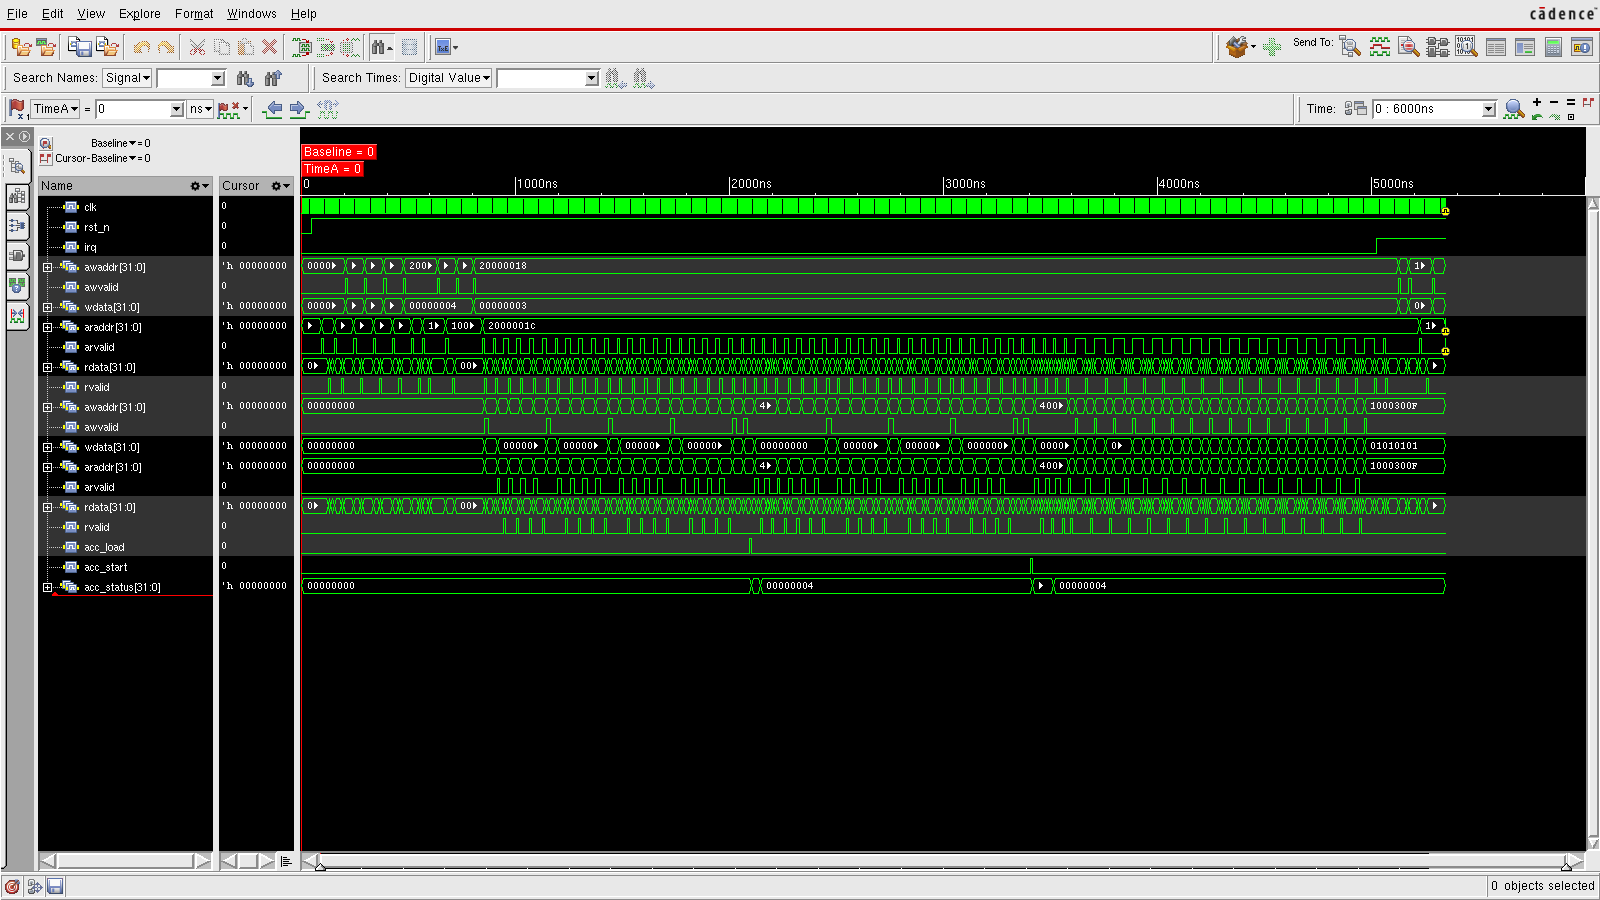
\includegraphics[height=0.74\textheight]{../../05.Verification/soc/evidencias/simvision_operacao_completa.png}

\scriptsize CPU programa o DMA e lê STATUS em laço; DMA lê $A$ e $B$ e escreve nos buffers; LOAD e
START na malha; escrita de $C$; \code{irq} sobe.
\end{frame}

% ---------------------------------------------------------------- 13
\begin{frame}{Limitações e próximos passos}
\small
\begin{itemize}
  \item A CPU ainda é o modelo comportamental. O firmware usa 8 instruções e só acesso de palavra,
  para o core real rodar sem mudança.
  \item A largura de $C$ segue o RTL (largura do elemento, com volta), como propõe a decisão
  0002; se mudar, muda um parâmetro (\code{+C_WIDTH}).
  \item A ligação do acelerador segue a proposta da decisão 0003 (decodificador local), conferida
  em teste de unidade: nenhum ciclo a mais.
  \item Endereços de $A$, $B$ e $C$ só múltiplos do tamanho do elemento.
  \item Sem IMC, não há cobertura de código.
\end{itemize}
\end{frame}

% ---------------------------------------------------------------- 14
\begin{frame}[fragile]{Roteiro da demonstração}
\footnotesize
\begin{enumerate}
  \item Compilação limpa: \code{make clean && make uvm-elab TB=soc}
  \item Teste dirigido: \code{make uvm TEST=mm_smoke_test} (topologia, scoreboard, veredito)
  \item Aleatório com a seed do professor: \code{make uvm TEST=mm_rand_test SEED=<seed>}
  \item Cobertura: \code{make uvm TEST=mm_tiling_test COV=1} e \code{make cov-merge}
  \item SimVision: \code{make uvm TEST=mm_smoke_test WAVES=1} e \code{make uvm-gui}
  \item Erro detectado: \code{make uvm TEST=mm_fault_test FAULT=fw_dim_k EXPECT=fail}
\end{enumerate}
\vspace{3mm}
\small Tudo a partir da raiz do repositório; o README do ambiente
(\code{05.Verification/soc/README.md}) traz os comandos e a lista de testes.
\end{frame}

\end{document}
